\chapter{Arquitectura do $\mu$RISC}
\section{Unidade de descodificação - Decoder}

Por decisão própria, na unidade de descodificação foi efectuado o máximo possível de descodificação de operações, selectores de \textit{multiplexers} e unidades funcionais. Desta forma é nos possível generalizar as restantes unidades funcionais centralizando toda a descodificação numa só unidade. Uma consequência desta metodologia é o aumento da complexidade da unidade e o número de sinais de \textit{output}.\par O mesmo método foi aplicado para as instruções de \textit{jump}. Uma descodificação parcial é feita no \textit{decoder} permitindo diminuir a lógica aplicada à unidade funcional de saltos.


\section{Unidade de Armazenamento - Memória RAM/ROM partilhada}

De forma a facilitar o endereçamento da memória optou-se por uma unidade de armazenamento partilhado. No início da simulação esta é inicializada a partir de um ficheiro .txt graças à utilização de uma \textit{impure function} que introduz as instruções a primeira posição de memória incrementando o endereço para a seguinte instrução. 
Esta unidade apresenta três entradas, Din para o armazenamento de dados através para instrução \textit{store}, Addr\_Instr que indica o endereço da próxima instrução a ser enviada para o \textit{Decoder} e Addr\_Dados que endereça a posição para onde será feito uma instrução de \textit{load}.
Como saídas tem-se Dout\_Dados proveniente da instrução \textit{load} e Instr que indica a próxima instrução.

As vantagens deste tipo de memória é a facilidade de endereçamento uma vez que não é necessário fornecer um offset para o caso em que é necessário aceder a um array \textit{por exemplo}. Como desvantagem tem se o facto de o programador necessitar de uma extra atenção às posições de memória onde guarda dos dados podendo substituir futuras instruções.

Com duas memórias independentes seria possível evitar este problema caso ambas as memórias fossem inicializadas com os mesmos dados (instruções e \textit{arrays}).

\section{Unidade lógico-aritmética - ALU}

Desenhou-se a ALU com três unidades a funcionarem em paralelo, abaixo descritas com maior detalhe.
O resultado produzido por estas unidades é introduzido num \textit{multiplexer} que selecciona de acordo com sinais provenientes da unidade de descodificação qual o resultado e as \textit{Flags} a colocar à saída da ALU.


\subsection{Unidade Aritmética}
A unidade Aritmética é responsável pelas operações apresentadas na tabela~\ref{tabela:arith}.

\begin{table}[h]
	\centering
	\begin{tabular}{|c|c|c|c|}
		\hline
		OP    & Operação & Mnemónica & Flags actualizadas \\ \hline
		00000 & \mbox{$C=A+B$}    & add c, a, b    & S,C,Z,V   \\ \hline
		00001 & \mbox{$C=A+B+1$}  & addinc c, a, b & S,C,Z,V   \\ \hline
		00011 & \mbox{$C=A+1$}    & inca c, a      & S,C,Z,V   \\ \hline
		00100 & \mbox{$C=A-B-1$}  & subdec c, a, b & S,C,Z,V   \\ \hline
		00101 & \mbox{$C=A-B$}    & sub c, a, b    & S,C,Z,V   \\ \hline
		00110 & \mbox{$C=A-1$}    & deca c, a      & S,C,Z,V   \\ \hline
	\end{tabular}
	\caption{Operações Aritméticas}
	\label{tabela:arith}
\end{table}

A unidade aritmética começa por analisar qual a operação a executar de acordo com os dados vindos da unidade de descodificação e em seguida começa por calcular o segundo membro da operação \mbox{$C=A+operB$} em que 
\[ operB=\left\{
\begin{array}{lr}
B & : OP=00000\\
B+1 & : OP=00001\\
1 & : OP=00011\\
-B-1 & : OP=00100\\
-B & : OP=00101\\
-1 & : OP=00110
\end{array}
\right.\]
De seguida calcula \mbox{$C=A+operB$} e as \textit{Flags} correspondentes com base na análise do resultado e dos operandos.

\subsection{Unidade Lógica}

A unidade Lógica é responsável pelas operações apresentadas na tabela~\ref{tabela:logic}.\\

\begin{table}[h]
	\centering
	\begin{tabular}{|c|c|c|c|}
		\hline
		OP    & Operação & Mnemónica & Flags actualizadas \\ \hline
		10000 & \mbox{$C=0$}    & zeros c   & Nenhuma  \\ \hline
		10001 & \mbox{$C=A\&B$}  & and c, a, b & S,Z   \\ \hline
		10010 & \mbox{$C=!A\&B$}  & andnota c, a, b & S,Z   \\ \hline
		10011 & \mbox{$C=B$}  & passb c, b &  Nenhuma  \\ \hline
		10100 & \mbox{$C=A\&!B$}  & andnotb c, a, b & S,Z   \\ \hline
		10101 & \mbox{$C=A$}  & passa c, a & S,Z   \\ \hline
		10110 & \mbox{$C=A \oplus B$}  & xor c, a, b & S,Z   \\ \hline
		10111 & \mbox{$C=A|B$}  & or c, a, b & S,Z   \\ \hline
		11000 & \mbox{$C=!A\&!B$}  & nor c, a, b & S,Z   \\ \hline
		11001 & \mbox{$C=!(A \oplus B)$}  & xnor c, a, b & S,Z   \\ \hline
		11010 & \mbox{$C=!A$}  & passnota c, a & S,Z   \\ \hline
		11011 & \mbox{$C=!A|B$}  & ornota c, a, b & S,Z   \\ \hline
		11100 & \mbox{$C=!B$}  & passnotb c, b & S,Z   \\ \hline
		11101 & \mbox{$C=!A|!B$}  & nand c, a, b & S,Z   \\ \hline
		11111 & \mbox{$C=1$}  & ones c & Nenhuma   \\ \hline
	\end{tabular}
	\caption{Operações de Deslocamento}
	\label{tabela:logic}
\end{table}
\newpage
\subsection{Unidade de Deslocamentos}
A unidade de Deslocamentos é responsável pelas operações apresentadas na tabela \ref{tabela:shift}.\\

\begin{table}[h]
	\centering
	\begin{tabular}{|c|c|c|c|}
		\hline
		OP    & Operação & Mnemónica & Flags actualizadas \\ \hline
		01000 & \mbox{$C=Shift Lógico Esq.(A)$}    & lsl c, a   & S,C,Z   \\ \hline
		01001 & \mbox{$C=Shift Aritmético Dir.(A)$}  & asr c, a & S,C,Z   \\ \hline
	\end{tabular}
	\caption{Operações de Deslocamento}
	\label{tabela:shift}
\end{table}

No caso do \textit{shift} lógico a saída resulta do deslocamento do sinal de entrada uma posição e preenchimento do \textit{bit0} com 0. No caso do \textit{shift} aritmético a saída resulta do deslocamento do sinal de entrada uma posição e preenchimento do \textit{bit15} com o \textit{bit15} da entrada.\\

\section{Unidade de Constantes}
A unidade de Constantes é responsável pelas operações apresentadas na tabela~\ref{tabela:constantes}.
\begin{table}[h]
	\centering
	\begin{tabular}{|c|c|c|}
		\hline
		Formato & Operação & Mnemónica \\ \hline
		I & \mbox{$C=Constante$} & loadlit c, Const  \\ \hline
		II & \mbox{$C=Const8|(C\&0xff00)$}  & lcl c, Const8 \\ \hline
		II & \mbox{$C=(Const8<<8)|(C\&0x00ff)$}  & lch c, Const8 \\ \hline
	\end{tabular}
	\caption{Operações com Constantes}
	\label{tabela:constantes}
\end{table}

Optámos por separar estas operações das restantes da ALU de modo a facilitar a descodificação das instruções por parte do \textit{Decoder} e uma vez que o caminho crítico é devido à elevada complexidade da ALU a separação desta unidade funcional da ALU não tem qualquer tipo de influência na frequência de relógio.

\section{Unidade de Controlo de saltos e \textit{flags}}
Desenhou-se a unidade de modo a controlar o próximo endereço a enviar ao \textit{Program Counter} (PC). Esta unidade guarda os valores das \textit{flags} provenientes da ALU em registos e depois usa esses registos para calcular as condições de salto.\par
Juntámos os registos das \textit{flags} com a unidade de controlo de saltos de modo a que consoante a condição de salto vinda do \textit{Decoder} se pudesse calcular se se deveria executar um salto ou se permitíamos que o valor do \textit{PC} fosse incrementado normalmente.\par
O cálculo do próximo endereço do \textit{PC} é feito em 4 fases.
\begin{enumerate}
	\setlength{\itemindent}{25pt}
	\item Cálculo da condição de salto
	\item Cálculo do \textit{offset} para o caso de saltos no Formato I ou do Formato II
	\item Determinar se o salto é para um \textit{offset} ou para um registo
	\item Determinar o próximo endereço do \textit{PC} com base no tipo de \textit{jump} (condicional ou incondicional) e a condição
\end{enumerate}

\[\text{Condição}=\left\{
\begin{array}{rcl}
1 & : & COND=0000\\
flagV & : & COND=0011\\
flagS & : & COND=0100\\
flagZ & : & COND=0101\\
flagC & : &  COND=0110\\
flagS+flagZ & : & COND=0111\\
0 & : & others
\end{array}\right.\]

\[\text{Offset}=\left\{
\begin{array}{rcl}
\begin{array}{r}
Destino(11) \&Destino(11) \&Destino(11) \&Destino(11)\\
\&Destino(11\ downto\ 0)
\end{array} & : & OP=10\\
\begin{array}{r}
Destino(7)\&Destino(7)\&Destino(7)\&Destino(7)\&Destino(7)\\
\&Destino(7)\&Destino(7)\&Destino(7)\&Destino(7\ downto\ 0)
\end{array} & : & others
\end{array}\right.\]

\[\text{Jump Address}=\left\{
\begin{array}{rcl}
RB & : & OP=11\\
PC+1+Offset & : & others
\end{array}\right.\]

\[\text{Próximo PC}=\left\{
\begin{array}{rcl}
Jump\ Address & : & enable\_jump=1\ \cdot\ (\text{Condição} \oplus OP(0))=1\\
Jump\ Address & : & enable\_jump=1\ \cdot\ OP(1)=1\\
PC+1 & : & others
\end{array}\right.\]

\section{Esquema da Arquitectura}

\begin{figure}[H]
	\begin{center}
		\makebox[\textwidth][c]{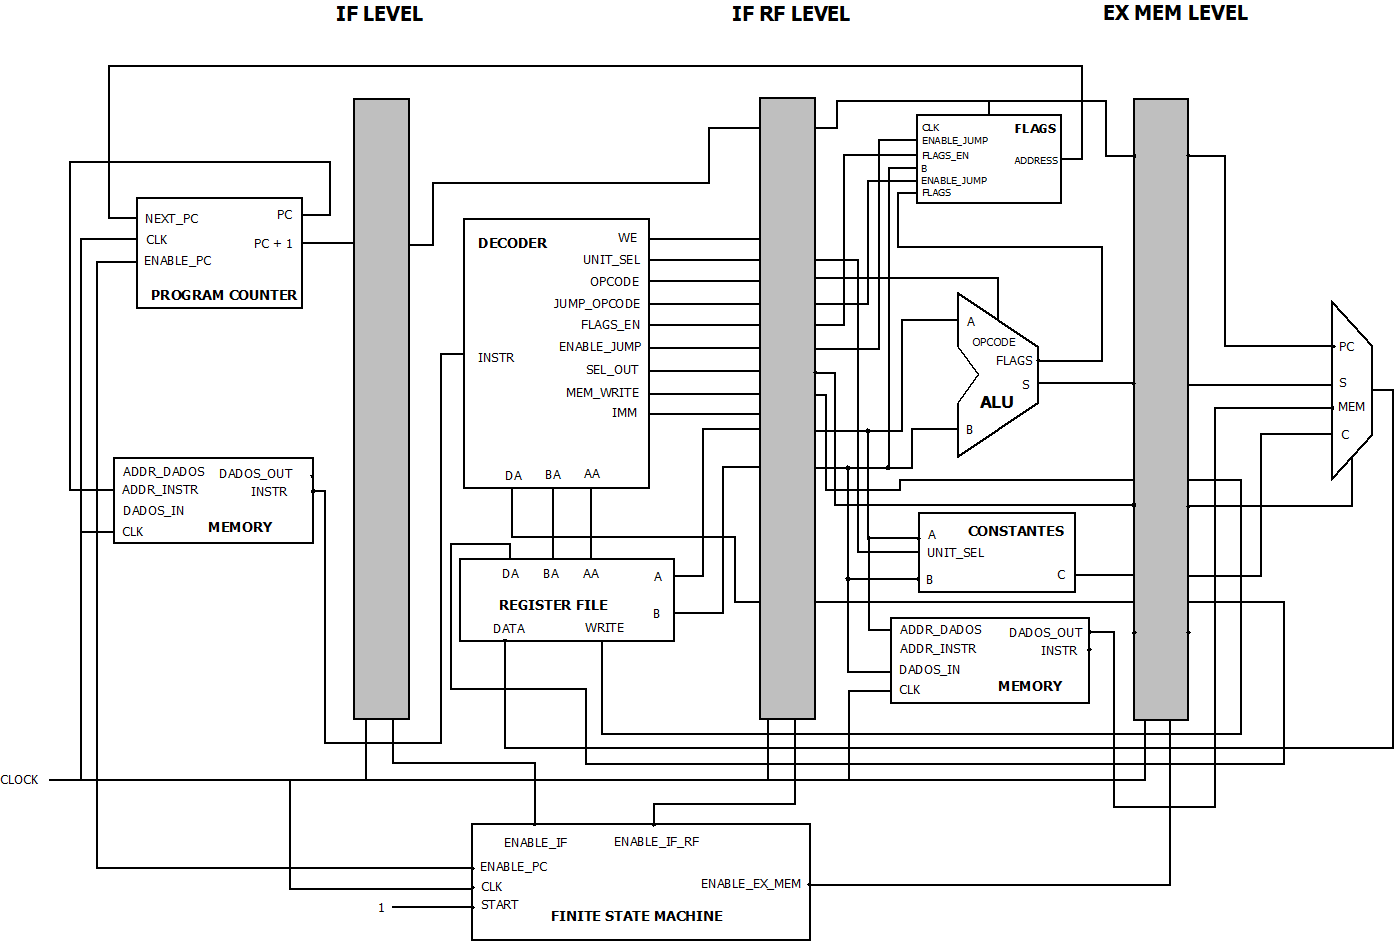
\includegraphics[clip, keepaspectratio=true, scale=0.42]{./images/CPU.png}}
		\caption{Arquitectura $\mu$RISC.}
		\label{arquit}
	\end{center}
\end{figure}